\documentclass[a3paper,landscape]{article}

\usepackage[french]{babel}
\usepackage[utf8]{inputenc}
\usepackage[T1]{fontenc}

\usepackage{graphicx}
\usepackage{multicol}
\usepackage{geometry}
\usepackage{xcolor}
\usepackage{amsmath}
\usepackage{booktabs}

\geometry{margin=0.1cm}
\pagestyle{empty}

\begin{document}

\begin{center}
{\Huge\bfseries Variables de contexte et réussite scolaire, Groupe D1\_B}\\[0.4cm]
\vspace{0.2cm}
\end{center}
\begin{multicols}{3}

% =========================
\section*{1. Problématique}

Dans quelle mesure les variables de contexte permettent-elles d'expliquer les différences de réussite scolaire et de prédire les résultats des élèves ?
Analyse des variables de contexte pour :

\begin{itemize}
\item prédire G3
\item classifier réussite / échec
\end{itemize}

G1 et G2 supprimées pour éviter fuite de données.

% =========================
\section*{2. ACP (Analyse en composantes principales)}

\begin{center}
\includegraphics[width=0.6\linewidth]{../Rapport/figures_rapport/acp_cercle.png}
\end{center}

\begin{center}
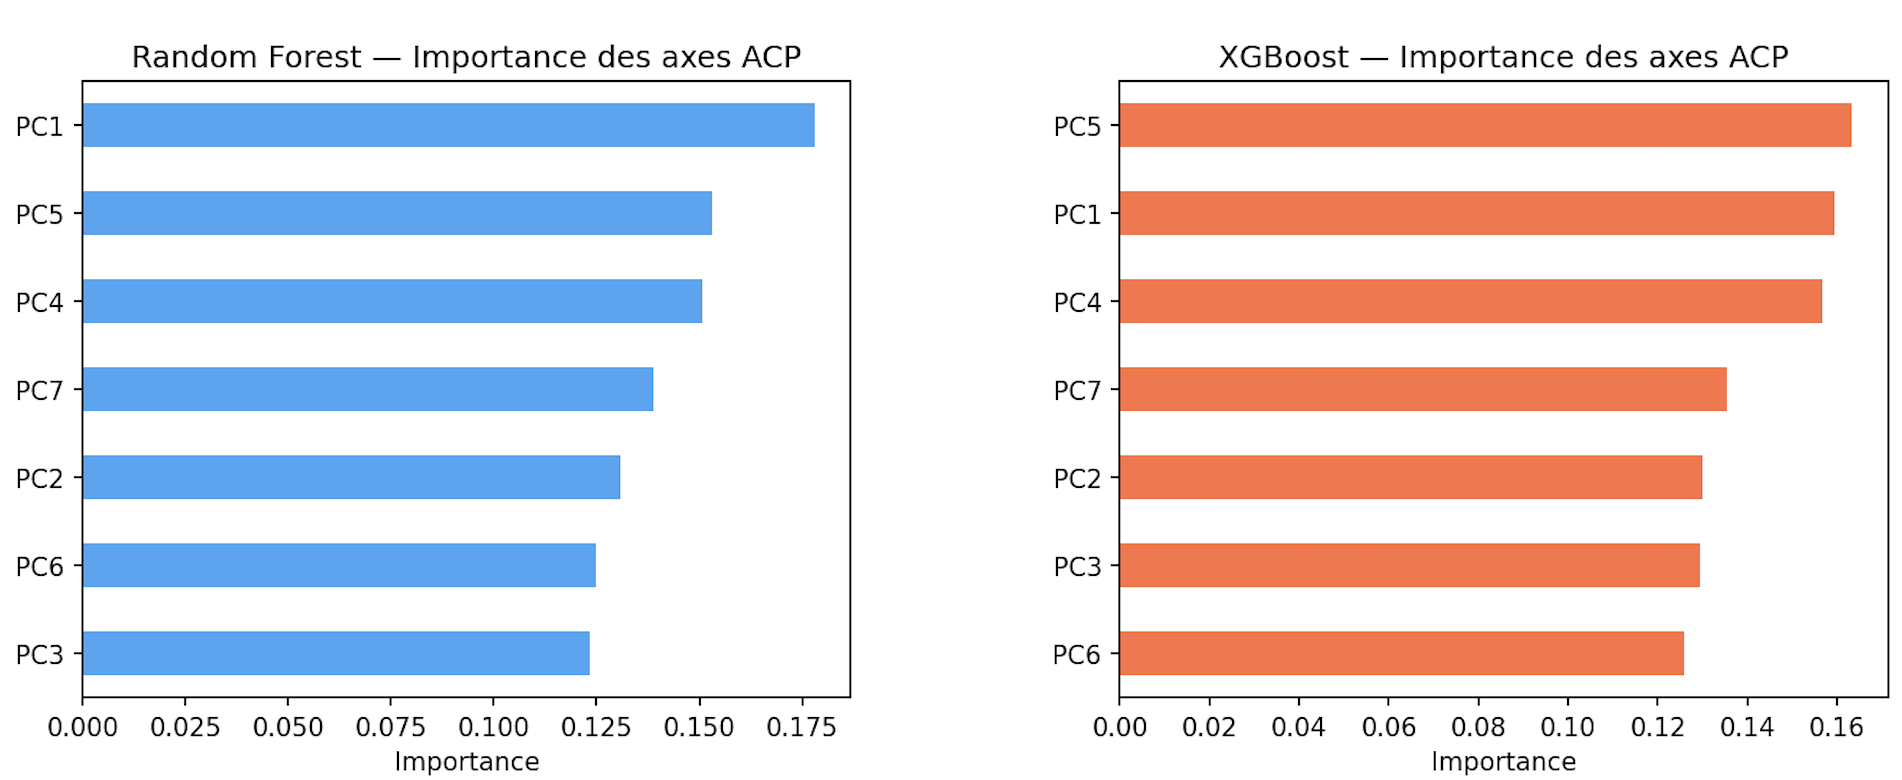
\includegraphics[width=0.6\linewidth]{../Rapport/figures_rapport/importance_axes_acp.png}
\end{center}

\textbf{Résultats :}
\begin{itemize}
\item corrélations fortes (Medu/Fedu, Dalc/Walc)
\item axe réussite vs risque
\item variables dominantes identifiées
\end{itemize}

% =========================
\section*{3. K-Means (clustering)}

\begin{center}
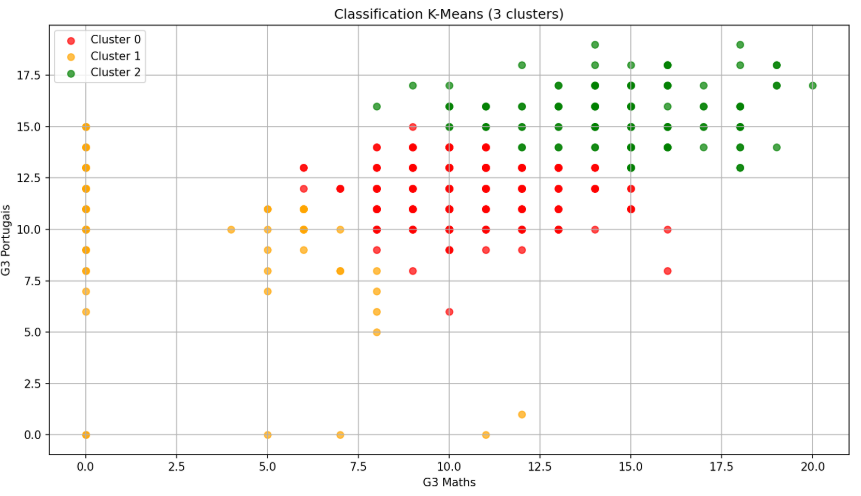
\includegraphics[width=0.55\linewidth]{../Rapport/figures_rapport/kmeans_notes.png}
\end{center}

\textbf{Résultat :}
\begin{itemize}
\item 3 groupes d’élèves
\item faible / moyen / fort
\end{itemize}

% =========================
\section*{4. Arbres de décision (variables originales)}

\begin{center}
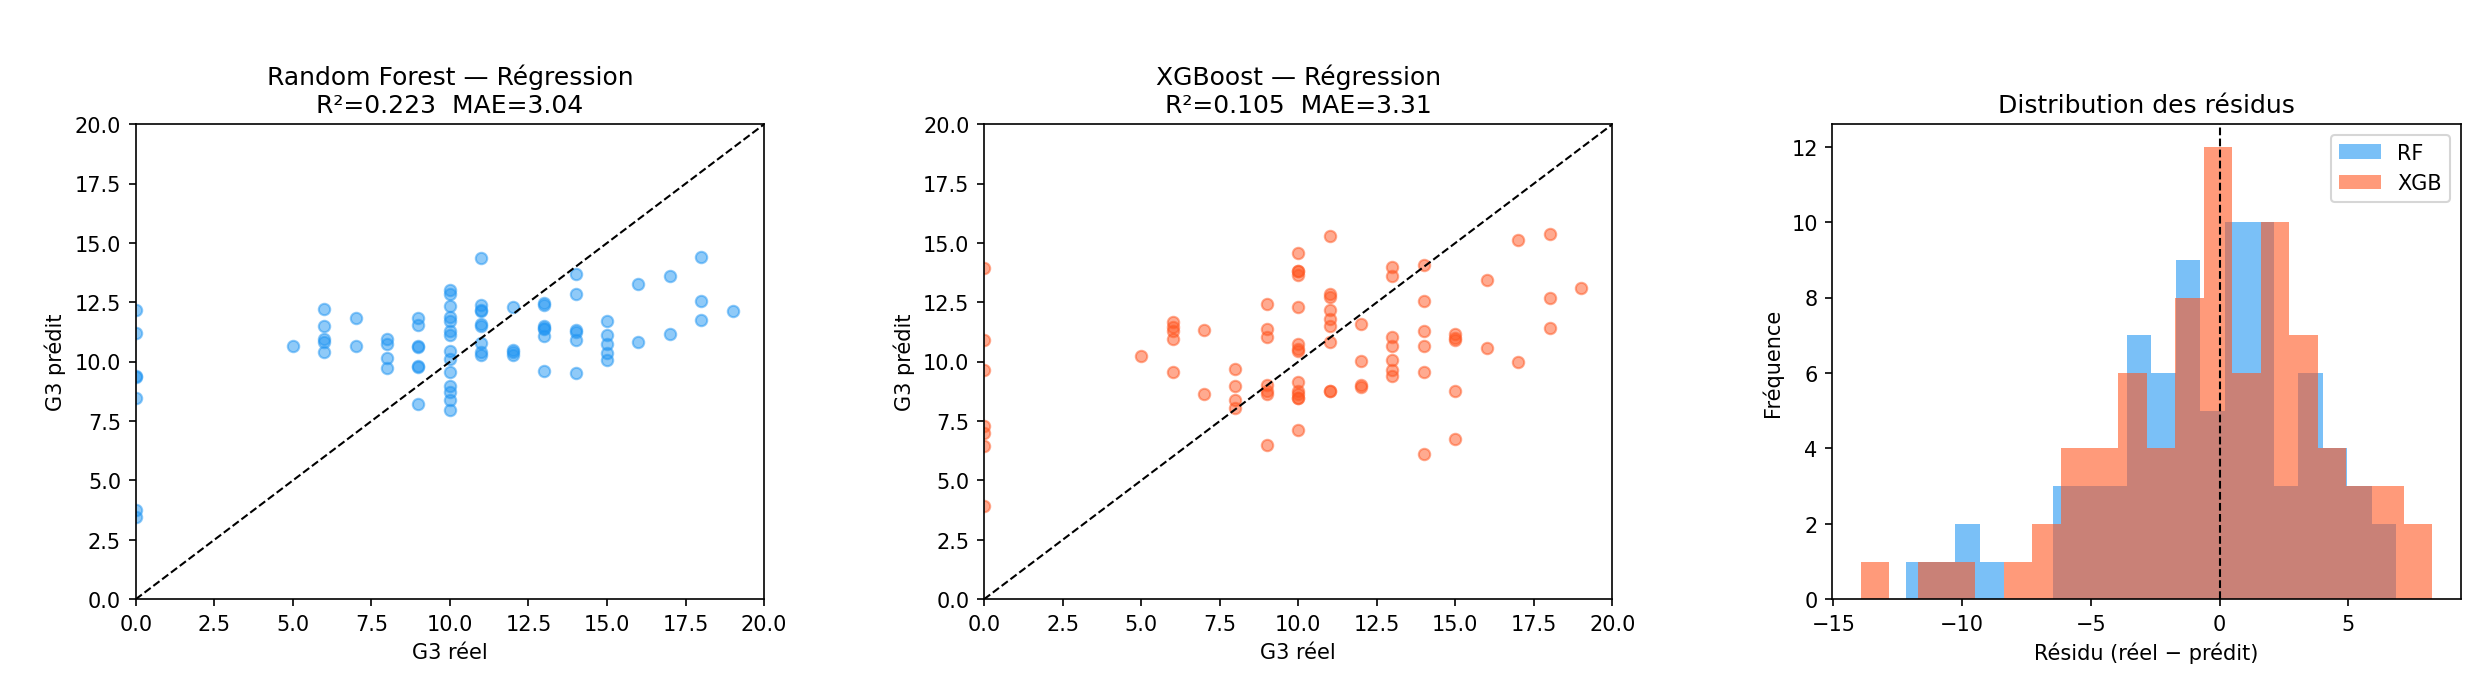
\includegraphics[width=1\linewidth]{../Rapport/figures_rapport/regression_arbres.png}
\end{center}

\begin{center}
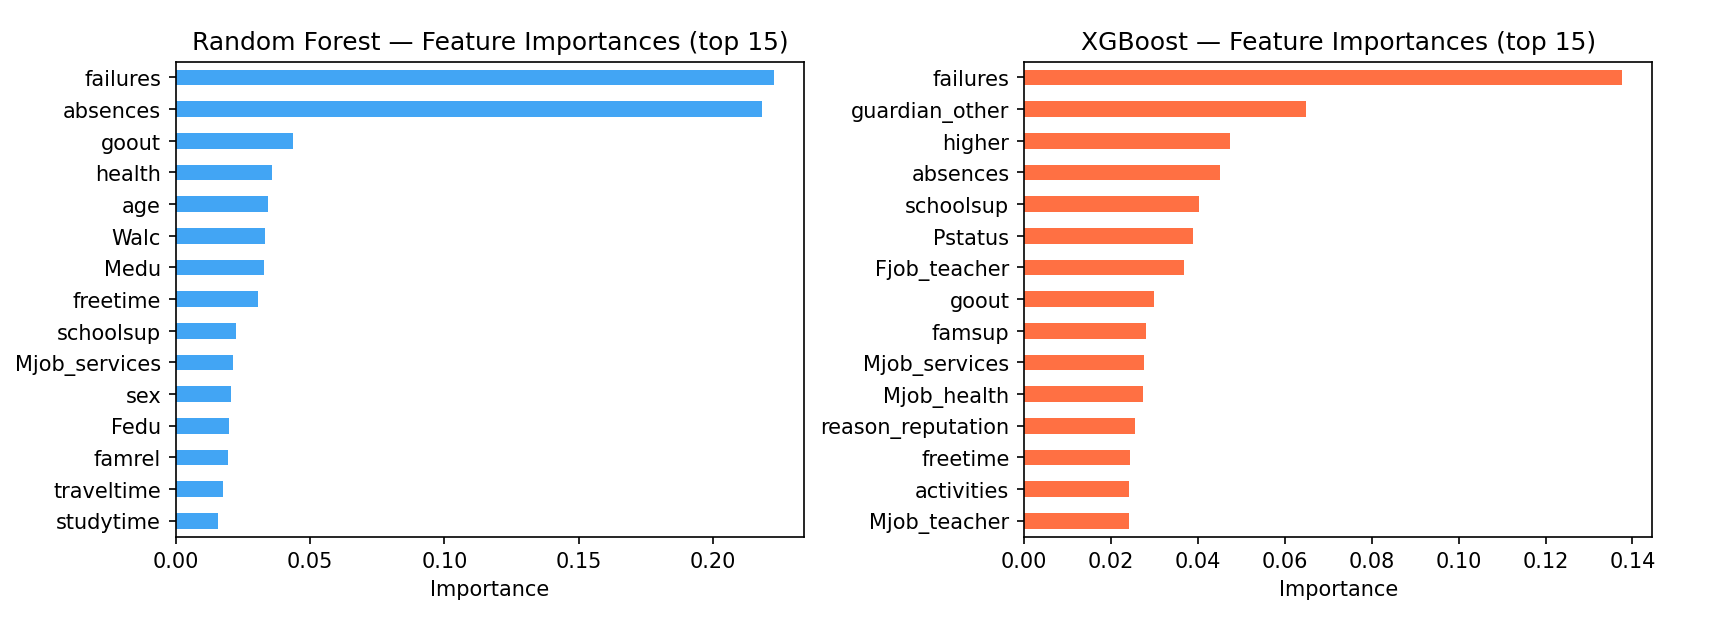
\includegraphics[width=.6\linewidth]{../Rapport/figures_rapport/importance_arbres.png}
\end{center}

\textbf{Régression :}

\begin{center}
\begin{tabular}{lc}
\toprule
Modèle & $R^2$ \\
\midrule
Random Forest & 0.223 \\
XGBoost & 0.105 \\
\bottomrule
\end{tabular}
\end{center}

\textbf{Variables importantes :}
failures, absences, higher, goout

% =========================
\section*{5. Classification (arbres)}

\begin{center}
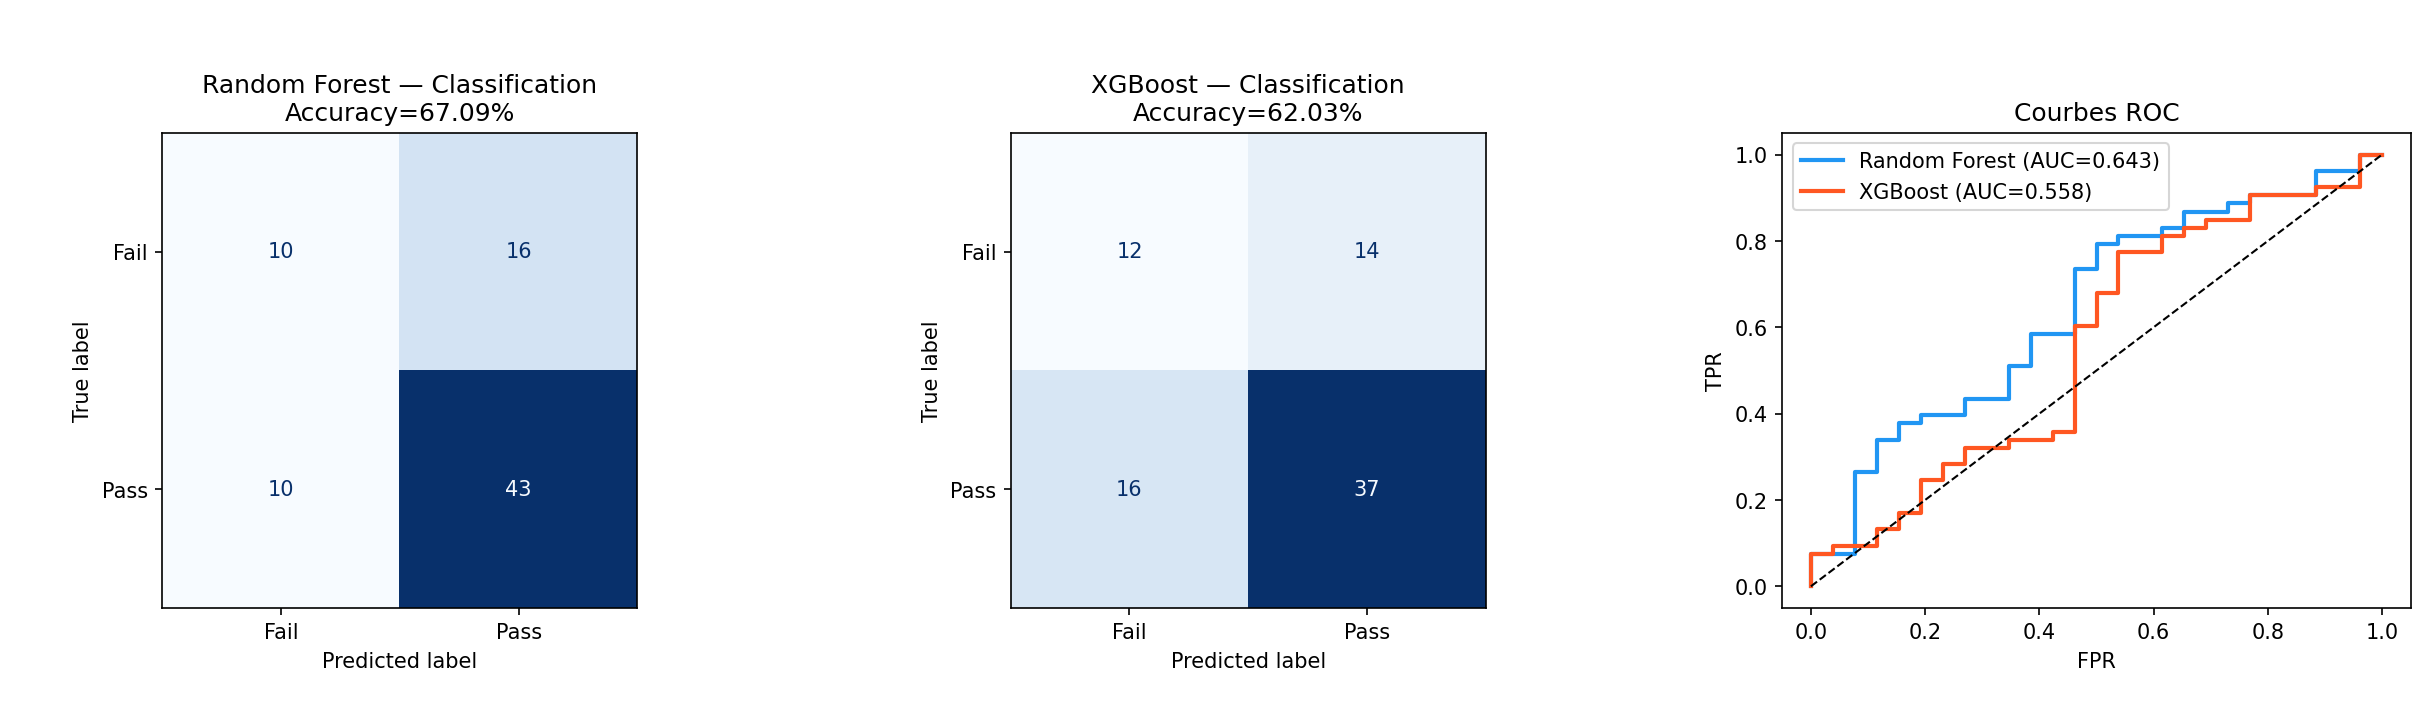
\includegraphics[width=1\linewidth]{../Rapport/figures_rapport/classification_arbres.png}
\end{center}

\begin{center}
\begin{tabular}{lc}
\toprule
Modèle & Accuracy \\
\midrule
Random Forest & 67\% \\
XGBoost & 62\% \\
LDA & 66\% \\
QDA & 66\% \\
\bottomrule
\end{tabular}
\end{center}

% =========================
\section*{6. ACP + classification}

\begin{center}
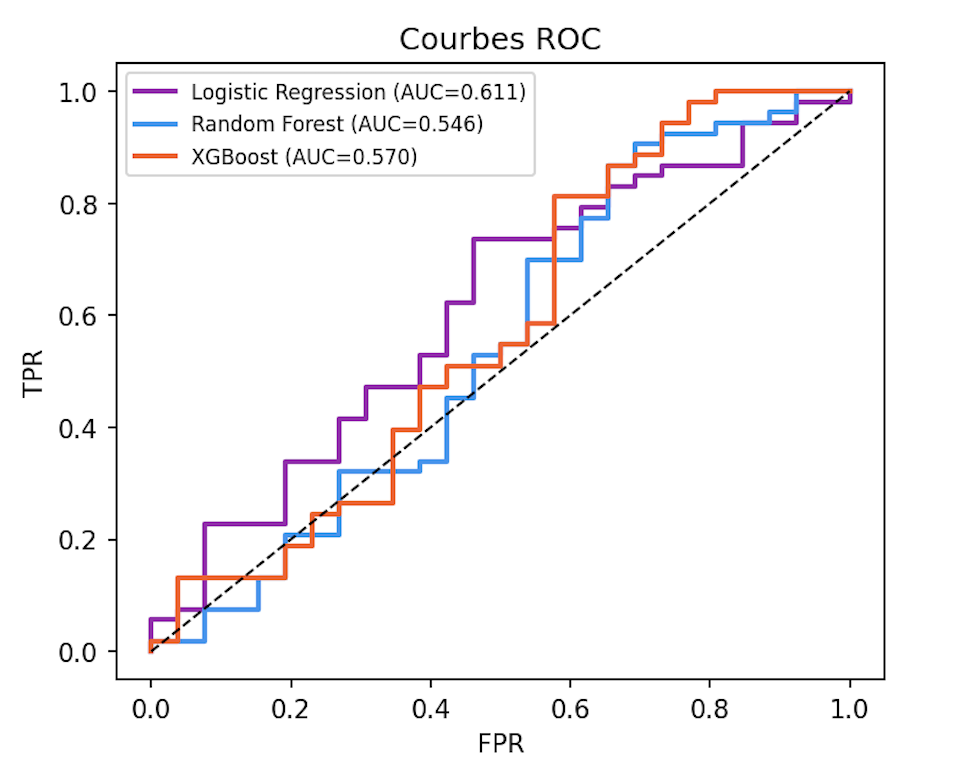
\includegraphics[width=0.6\linewidth]{../Rapport/figures_rapport/classification_acp_roc.png}
\end{center}

\begin{center}
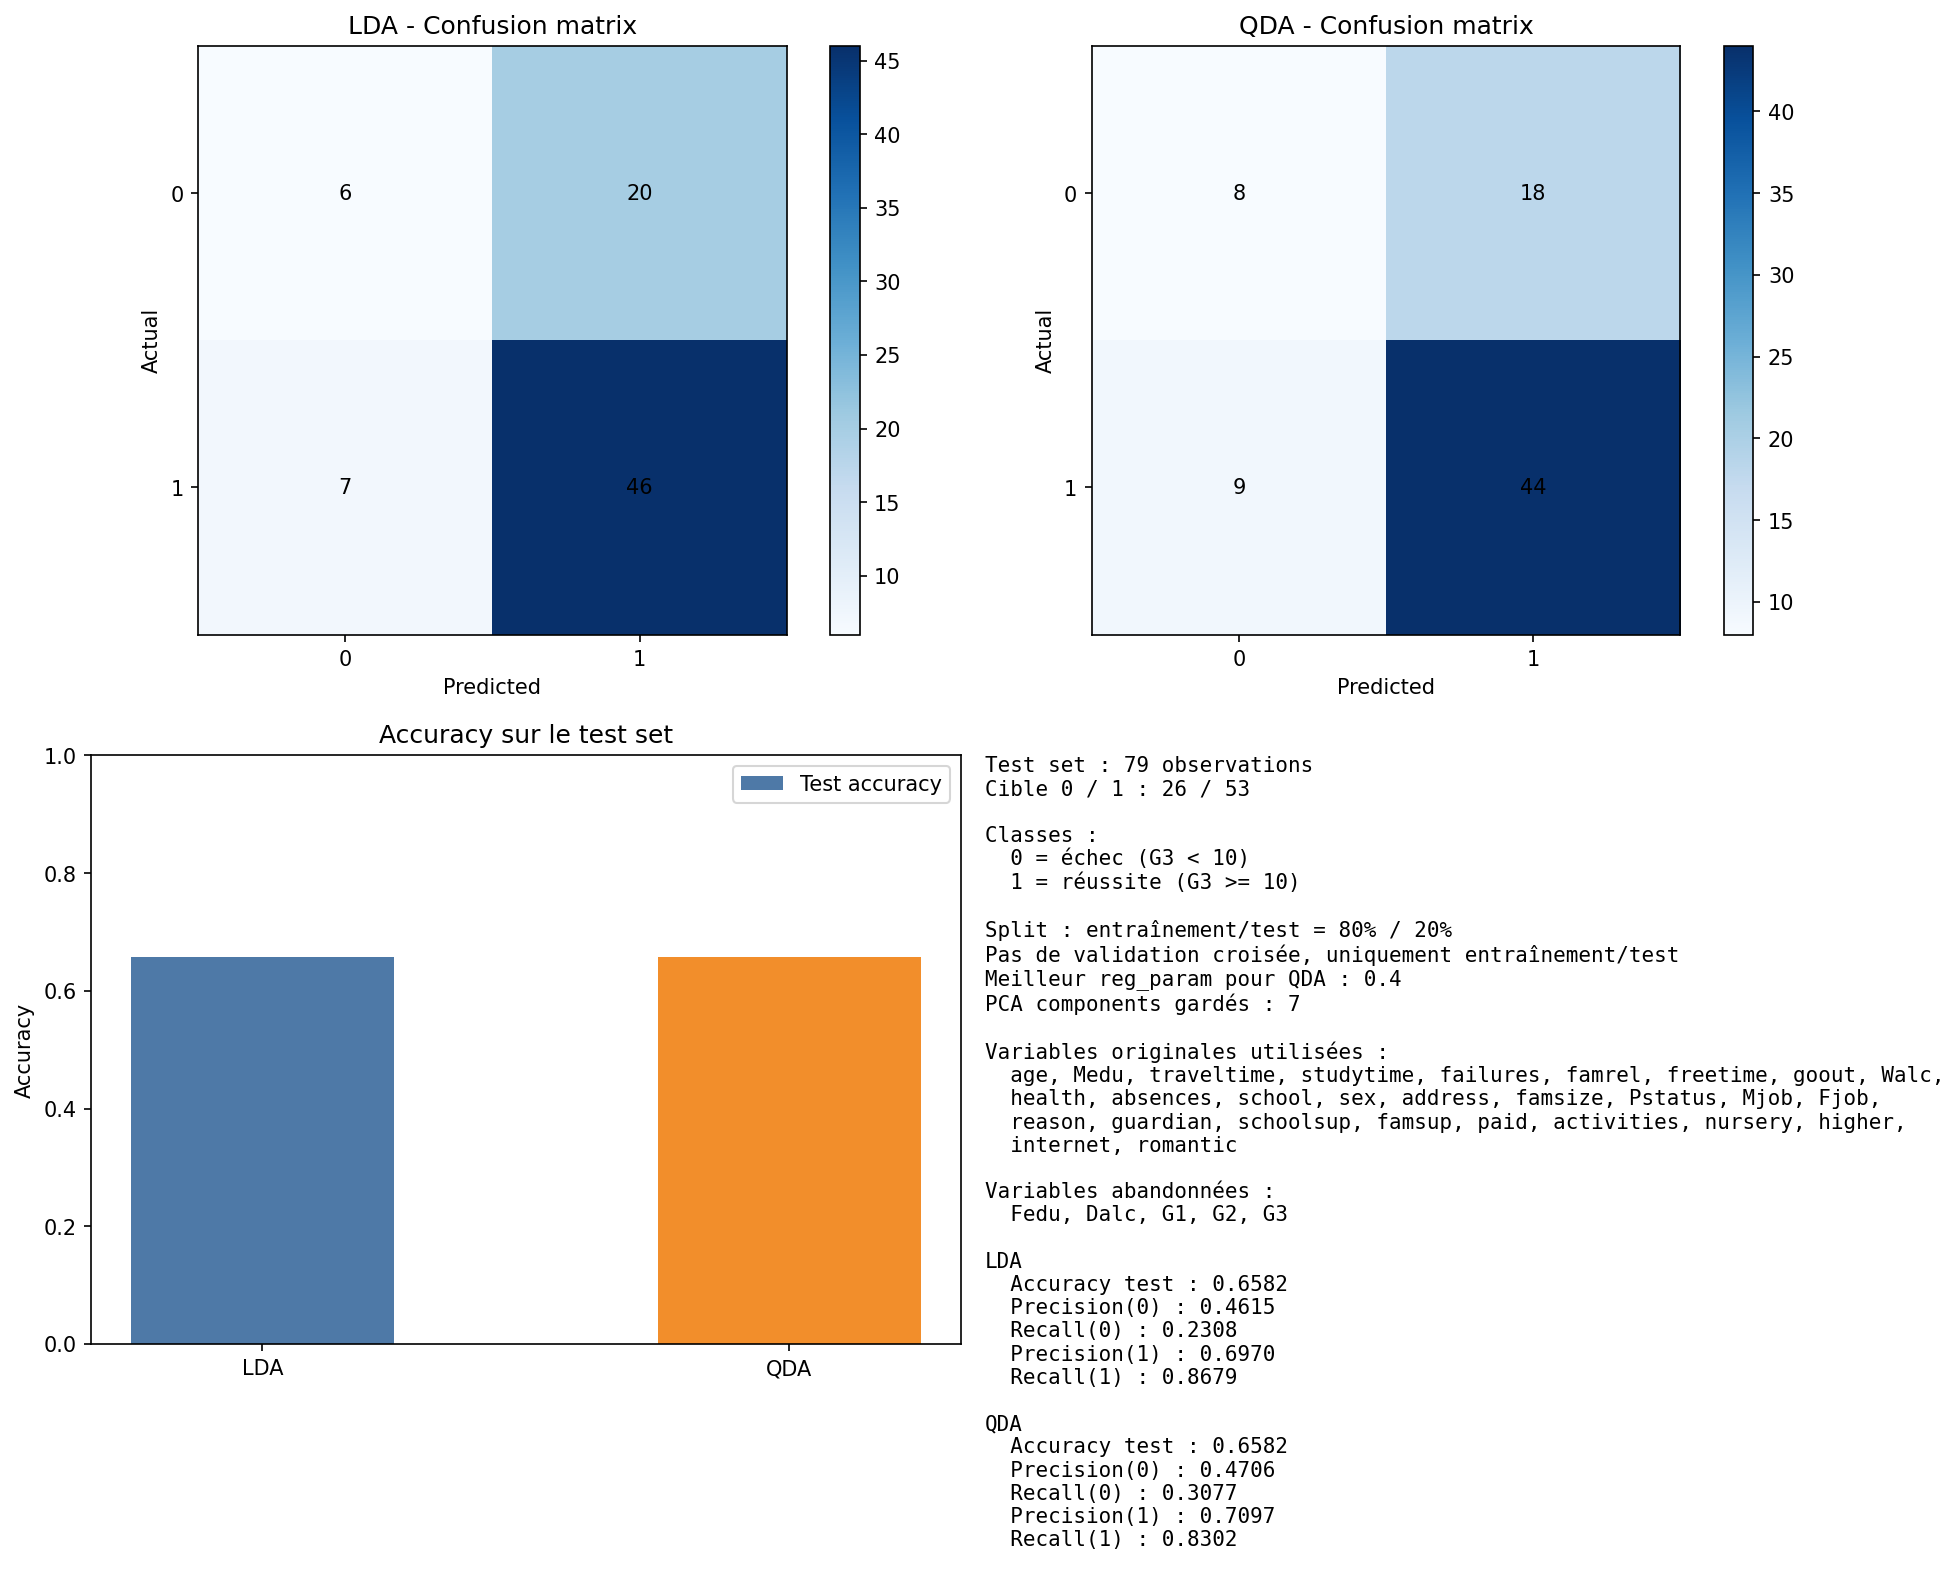
\includegraphics[width=1\linewidth]{../Rapport/figures_rapport/discriminante_acp.png}
\end{center}

\textbf{Conclusion :}
\begin{itemize}
\item légère amélioration des modèles linéaires
\item arbres peu sensibles à ACP
\item séparation classes visible mais imparfaite
\end{itemize}

% =========================
\section*{7. Régression avec ACP}

\begin{center}
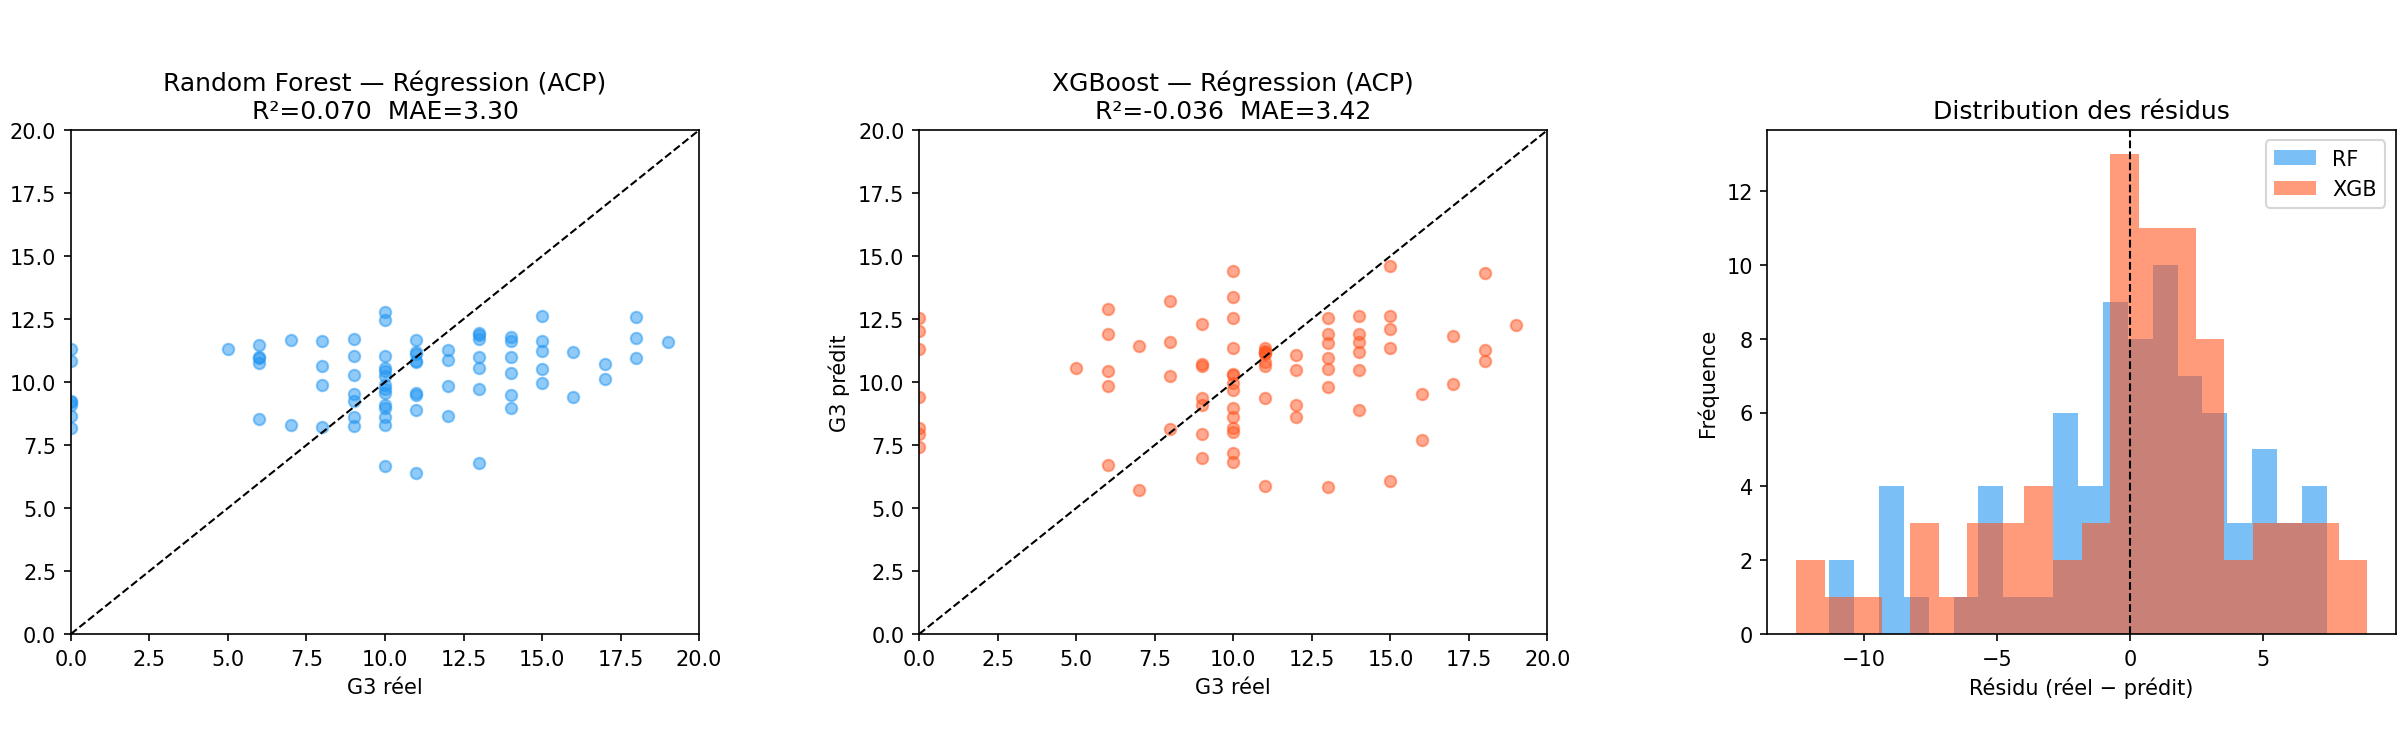
\includegraphics[width=1\linewidth]{../Rapport/figures_rapport/regression_acp.png}
\end{center}

\textbf{Observation :}
\begin{itemize}
\item stabilité faible des gains
\item perte d’interprétation directe
\end{itemize}

% =========================
\section*{Conclusion}

\begin{itemize}
\item signal réel dans les variables de contexte
\item performance limitée sans G1/G2
\item classification ~65-68\%
\item ACP utile pour structure, pas pour performance pure
\end{itemize}

\end{multicols}

\end{document}